\chapter{Evaluation}
\label{ch:evaluation}
The hclm cluster was used to evaluate the usability and performance of DIIS for mixing the self-energy. We decided to use reasonably small calculations that would finish in a few hours.

For each testing, we considered a square-lattice Hubbard model at interaction $U=8t$ and temperature $T=t/50$, where $t$ is the hopping amplitude.

\lstdefinelanguage{ini}{
  basicstyle=\ttfamily\small,
  columns=fullflexible,
  morecomment=[s][\color{Orchid}\bfseries]{[}{]},
  morecomment=[s][\color{Orchid}\bfseries]{[[}{]]},
  morecomment=[l]{\#},
  morecomment=[l]{;},
  commentstyle=\color{gray}\ttfamily,
  morekeywords={},
  keywordstyle={\color{green}\bfseries}
}

\begin{lstlisting}[label=lst:w2dyn_config, language=ini, caption=The w2dynmaics configuration for this case]
[General]
DOS=ReadIn
HkFile=hubbard_2d_80_80_1.hk
beta=50.
NAt=1
totdens=1.
EPSN=0
mu=4.0
DMFTsteps=50
StatisticSteps=0
FileNamePrefix=square_u08_b50_diis
magnetism=para
siw_moments=estimate
FTType=none
mixing=0.0
mixing_strategy=diis
mixing_diis_history=5
mixing_diis_period=1

[Atoms]
[[1]]
Hamiltonian=Density
Udd=8.0
Nd=1

[QMC]
Nwarmups=1e6
Nmeas=1e5
NCorr=200
Ntau=1000
Niw=2000
Eigenbasis=1 
MeasGiw=1
\end{lstlisting}

The reference was given by the same configuration, but without DIIS mixing. It was important to compare the results with and without DIIS to see if they agree. Different results would be a hint to a bug in the implementation or that DIIS is not applicable for these inputs or DMFT in general. The configuration file is given in listing \ref{fig:eval-diis-u8}.

\begin{figure}[H]
    \centering
    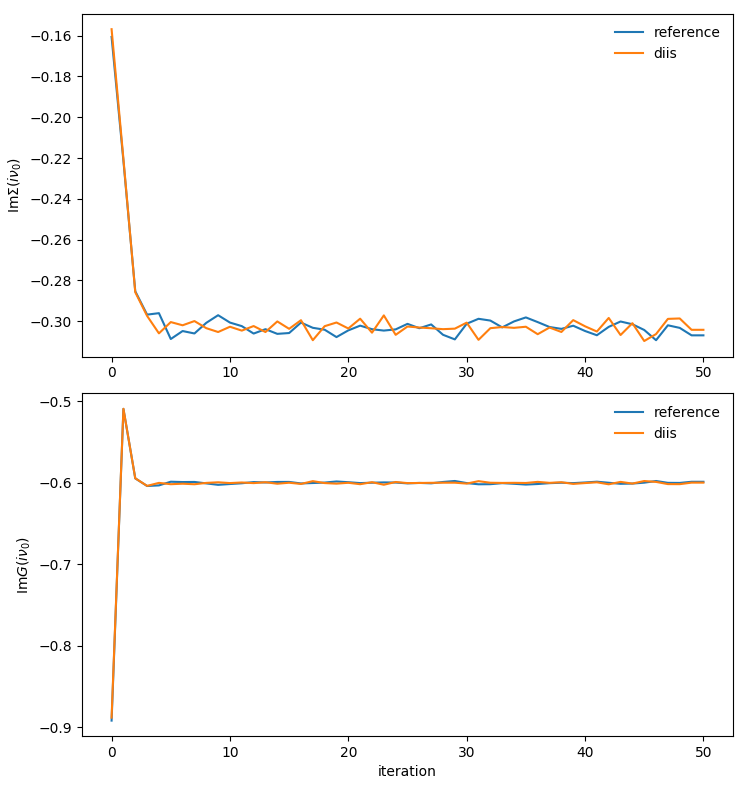
\includegraphics[width=1.0\textwidth]{figures/square_u08_b50_siw_imag_giw_imag.png}
    \caption{DMFT iteration comparison for Matsubara frequency $\pi/\beta$ and $U=8t$}
    \label{fig:eval-diis-u8}
\end{figure}

\begin{figure}[H]
    \centering
    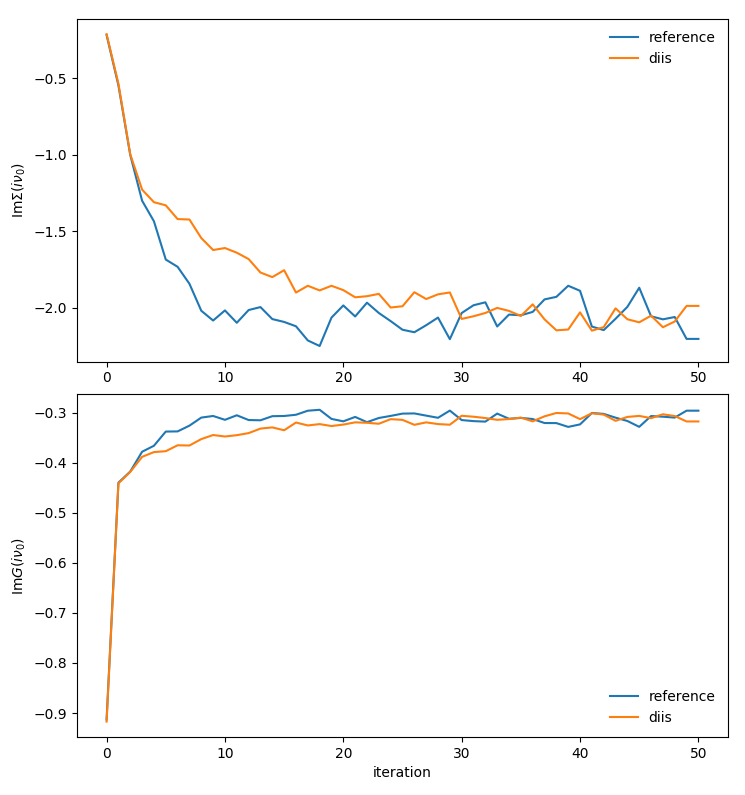
\includegraphics[width=1.0\textwidth]{figures/square_u12_b50_siw_imag_giw_imag.png}
    \caption{DMFT iteration comparison for Matsubara frequency $\pi/\beta$ and $U=12t$}
    \label{fig:eval-diis-u12}
\end{figure}

We can see that in figure \ref{fig:eval-diis-u8} that the result is the same with and without mixing while the rate of convergence is very similar.

A higher $U$ in figure \ref{fig:eval-diis-u12} shows a slower convergence in case of DIIS while the result is still the same. We are assuming that this is caused by the QMC noise. The DIIS appears to suppress this noise. A recent implementation of symmetric improved estimators\cite{symmetric} by Josef Kaufmann is promising better performance with DIIS.

